\section{Exercises}
	\subsection{Input and Output}
		\textbf{Make sure you're using IDLE for Python 3 here.}

		Input and output are fundamental features of almost any programming language and Python is no exception. Python provides us with a simple set of functions to handle input and output, named \texttt{input}, \texttt{raw\_input} (Python 2 only) and \texttt{print}.

		\lstinputlisting[style=Python, numbers=none]{McrRaspJam/014_Python/3_exercises/io.py}

		This example asks the user for their name, stores their input in a variable and then prints it out.

		\textbf{Extra:} Why not try asking for the user's favourite colour too?

		\begin{aside}[\texttt{input} and Python 2/3]
			In Python 2, the \texttt{input} function actually \textit{runs} the text that the user inputs, as opposed to just returning it into the variable. \texttt{raw\_input} actually returns the value the user inputs instead of running it. In Python 3 the \texttt{input} function replaces Python 2's \texttt{raw\_input} and \texttt{raw\_input} does not exist. You can try this out by running the above example and entering \texttt{3 + 4} as your name!
		\end{aside}

	\subsection{Randomness}

		Randomness can be found everywhere in programming, whether it be to work out where to put an enemy in Mario or even find $\pi$!

		\lstinputlisting[style=Python, numbers=none]{McrRaspJam/014_Python/3_exercises/randomness.py}

		\textbf{Extra:} Why not try modifying this code to print a random number between 0 and 1000?

		\begin{aside}[\texttt{random}]
			Python's random library provides a wide range of functions that return random values. Some examples are \texttt{random.random()} which returns a random number between 0 and 1, \texttt{random.getrandbits} which returns a number of random bits and \texttt{random.choice}, which returns a random item from a list.
		\end{aside}

	\subsection{Turtle}

		Python provides a library called \texttt{turtle}, which allows us to move a little robot around a virtual world! It's designed to be easy to use and uses plain English for all of it's commands, making it great to play around with.

		To get going with Python's \texttt{turtle}, we first need to import it so that we can use it's functions.

		\lstinputlisting[style=Python, numbers=none]{McrRaspJam/014_Python/3_exercises/turtle/import.py}

		Running this code won't do anything, as we need to move our turtle before a window opens.

		\begin{aside}[Opening the Window]
			You can get a window to open without a turtle by calling \texttt{turtle.setup()}. This function also allows you to set the size of the window and the starting position of the turtle.
		\end{aside}

		Our turtle can only go forwards and turn, so if we want to move in a different direction then we need to turn and face that direction. Our turtle always starts off facing to the right, so in the example below we'll move the turtle to the right a bit.

		\lstinputlisting[style=Python, numbers=none]{McrRaspJam/014_Python/3_exercises/turtle/move.py}

		\begin{center}
			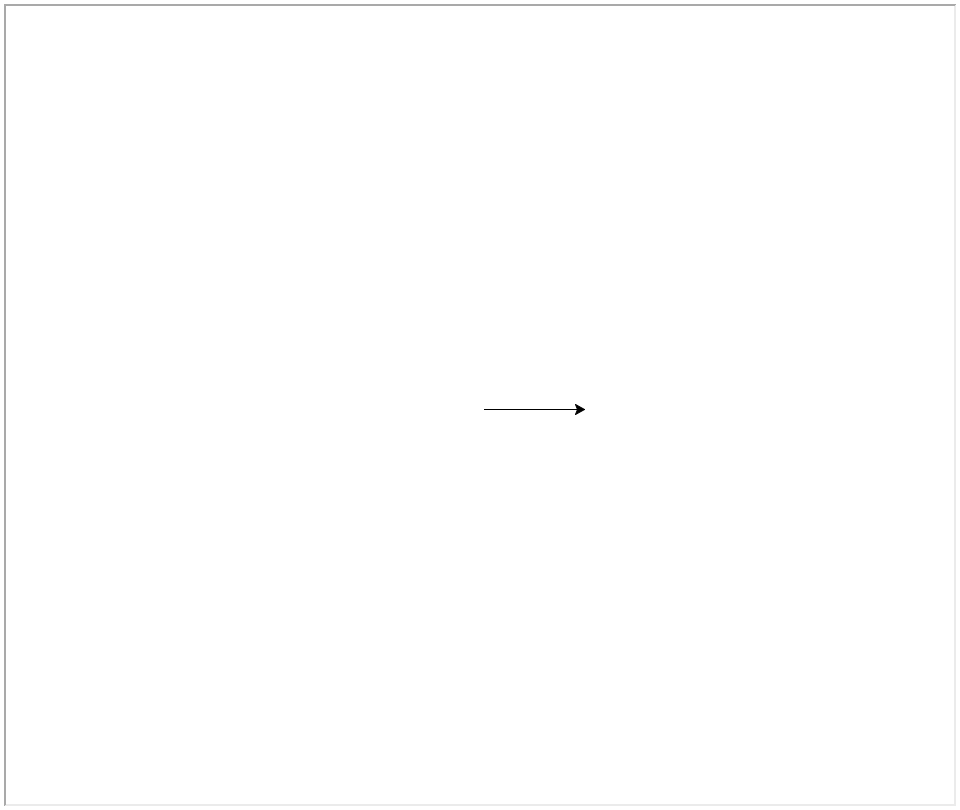
\includegraphics[width=100mm]{McrRaspJam/014_Python/3_exercises/turtle/move}
		\end{center}

		\begin{aside}[IDLE turtles]
			\texttt{turtle} works great in IDLE, as IDLE remains open even after you finish entering your code. Running Python code without IDLE is a different story, as Python exits once it reaches the end of your program! This means that the window will close after your turtle has finished moving, which is not what you want. An easy way to fix this is to add \texttt{turtle.mainloop()} at the very end of your code, which ensures that your program keeps running until you click the close button.
		\end{aside}

		\webclearpage

		We can also turn our turtle left and right by a certain number of degrees, and joined with our ability to move the turtle in the direction it's facing means we can move in direction! In the example below we draw a rectangle and end up back where we started.

		\lstinputlisting[style=Python, numbers=none]{McrRaspJam/014_Python/3_exercises/turtle/turn.py}

		We can use this alongside what we learned earlier about variables and loops to draw a hexagon!

		\lstinputlisting[style=Python, numbers=none]{McrRaspJam/014_Python/3_exercises/turtle/hexagon.py}
